\documentclass[10.5pt]{scrarticle}
\usepackage[utf8]{inputenc}
\usepackage[parfill]{parskip}
\usepackage[T1]{fontenc}
\usepackage[ngerman]{babel}
\usepackage{multirow}
\usepackage{placeins}
\usepackage[official]{eurosym}
\usepackage{listings}
\usepackage{geometry}
\usepackage{graphicx}
\usepackage{tabularx}
\usepackage{makecell}
\usepackage{courier}
\usepackage[many]{tcolorbox}
\geometry{a4paper, margin=2.5cm}
\graphicspath{ {./images/} }

\renewcommand{\familydefault}{\sfdefault}

\newtcolorbox{infobox}[1][]{
  breakable,
  title=#1,
  colback=white,
  colbacktitle=white,
  coltitle=black,
  fonttitle=\bfseries,
  bottomrule=1pt,
  toprule=1pt,
  leftrule=1pt,
  rightrule=1pt,
  titlerule=0pt,
  arc=0pt,
  outer arc=0pt,
  colframe=black,
}

\title{Entwicklung eines webbasierten ePortfolios}
\subtitle{im Rahmen einer Umschulung zum Fachinformatiker - Anwendungsentwicklung}
\author{Moritz Mandler \& Didier Zielke}
\date{\today}

\begin{document}
\lstset{
frameround=fttt,
numbers=left,
breaklines=true,
xleftmargin=0.75cm,
basicstyle=\ttfamily,
numberstyle=\ttfamily,
extendedchars=true,
inputencoding=utf8
}

\maketitle

%Hier müssen noch weitere Daten rein (siehe Merkblat der HK Hamburg):
%Berufsbezeichnung, Ausbilder, Ausbildungsbetrieb (mit Adresse)

\vspace{\fill}
\textbf{Prüflingsnummer:} \newline
XXX.XXX.XXX

\textbf{Ausbildungsbetrieb:}\newline
BFW Berufsförderungswerk Hamburg \newline
Marie-Bautz-Weg ??? \newline
22159 Hamburg

\textbf{Ausbilder:}\newline
Frau Treubel \newline
Herr Dr. Kubillus

\newpage

\tableofcontents

\newpage

\section{Einführung}

Die IT-Solution \& Design GmbH ist eine Lernfirma innerhalb des Berufsförderungswerks Hamburg GmbH (BFW). Als norddeutsches Zentrum für berufliche Rehabilitation und Integration ist das BFW Hamburg kompetenter Partner für Unternehmen, Träger der beruflichen Rehabilitation und Versicherungen und vor allem für Menschen, die aus gesundheitlichen Gründen ihre bisherige Tätigkeit nicht mehr ausüben können.  
Es soll eine einfache Plattform zur Veröffentlichung einer 'Mappe' der eigenen Arbeitsergebnisse geboten werden. Benutzer müssen sich authentifizieren und können dann die eigene Mappe bearbeiten. Innerhalb dieser Mappe, die hier nur eine Webseite darstellt, können beliebige Download-Dateien, Texte und Bilder eingefügt werden. So soll den Benutzern auch die Möglichkeit gegeben werden Lebensläufe, Arbeitsproben oder Zertifikate auf der eigenen Seite abzulegen.
Die IT-Solutions \& Design hat vom BFW Hamburg den Auftrag erhalten diese Webanwendung zu erstellen. 

\section{Projektdefinition}
\subsection{Ist-Analyse}

Die Teilnehmer*innen des BFW müssen sich während ihrer Ausbildung auf einen Praktikums- und einen Arbeitsplatz bewerben. Viele Bewerbungen werden dabei per E-Mail versendet. Um eine E-Mail nicht zu gro{\ss} werden zu lassen, werden dabei manchmal Arbeitsergebnisse, Zertifikate o. ä. nicht mit gesendet. Das könnte den Gesamteindruck im Bewerbungsprozess verschlechtern.  
 Au{\ss}erdem müssen die Teilnehmer*innen entscheiden, auf welche Unterlagen, Arbeitsproben und Bilder sie verzichten wollen.
 
\subsection{Anforderungsdefinition (Soll-Konzept}

Wie im Pflichtenheft angegeben (siehe Anhang) sollen folgende Anforderungen erfüllt werden:

\paragraph{i. Musskriterien}

\begin{itemize}
\item Neuanlegen, Ändern und Löschen von Benutzern durch den Admin
\item Jedem Benutzer ist eine Benutzerseite zugeordnet, die nur von dem jeweiligen Benutzer bearbeitet werden darf
\item Neuanlegen, Ändern und Löschen von Texten (auch Links) auf der jeweiligen Benutzerseite
\item Hochladen von Bildern und Pdf-Dateien innerhalb der Benutzerseite
\item Berücksichtigung verschiedener Berechtigungsstufen (Admin, Benutzer, Gast)
\item  Nur registrierte Gäste dürfen die Inhalte der Benutzer einsehen. Anlegen eines Gasts über Formular mit Überprüfung der E-Mailadresse (Freischaltung des Gastaccounts über E-Mail-Link) und Versenden eines generierten Kennworts 
\end{itemize}

\paragraph{ii. Wunschkriterien}

\begin{itemize}
\item Gäste dürfen nur die Portfolios sehen, welche ihnen über eine Freigabe zugeordnet wurden.
\end{itemize}

\paragraph{iii. Abgrenzungskriterien}

\begin{itemize}
\item Keine Überprüfung auf Verletzung von Urheberrechten oder Verstö{\ss}e gegen das    Datenschutzgesetz
\end{itemize}


\section{Projektplanung}
\subsection{Ressourcenplanung}
Als Ressource sollen ein PC mit der im Pflichtenheft angegebenen technischen Produktumgebung zur Verfügung gestellt werden. Für die Kalkulation wurde eine Stundenplanung gemacht. Zwei Personen sollen dem Projekt für die folgenden Arbeitsschritte zur Verfügung stehen.


%Die Tabelle steht auf der nächsten Seite, weil sie nicht "abgeschnitten" wird. 
\FloatBarrier
\begin{table}[ht!]
\begin{tabular}{lcr}
    \multicolumn{3}{l}{\textbf{Software-Entwurf}}\\
    Use-Case-Diagramm& &4h\\
    Klassenmodell & & 4h\\
    Datenmodell & & 4h\\
    \hline
    Summe: & & 12h\\
    \\
    \multicolumn{3}{l}{\textbf{Realisierung}}\\
    Entwurf der Testfälle & &  4h\\
    Programmierung Geschäftslogik& &  24h\\
    Programmierung Datenzugriffsklassen	& &  10h\\
    Programmierung Controller-Klassen& &  24h\\
    Programmierung View-Klassen& &  20h\\
    \hline
    Summe: & & 82h\\
    \\
    \multicolumn{3}{l}{\textbf{Tests}}\\
    Testfälle programmieren und durchführen& &10h\\
    Eventuelle Fehlerbeseitigung& &4h\\
    \hline
    Summe: & &\\
    \\
    \multicolumn{3}{l}{\textbf{Abschluss}}\\
    Soll-Ist-Vergleich& & 6h\\
    Dokumentation& & 25h\\
    Übergabe & & 1h\\
    \hline
    Summe: & &32h\\
   \textbf{Gesamtsumme:} & &\textbf{ 140h}

\end{tabular}
\end{table}
\FloatBarrier


\subsection{Kosten}

Die Kosten für dieses Projekt belaufen sich bei einem Stundensatz von 35,00\euro{} und einem Gesamteinsatz von 140Std. pro Person, wie aus der Ressourcenplanung hervorgeht, auf:

2 Personen * 140Std * 35,00\euro{} 				= \textbf{9800\euro{}}

\section{Projektdurchführung}
\subsection{Softwareentwurf}

Zuerst werden die Anwendungsfälle ermittelt. Es wird drei Hauptanwendungsfälle geben. Die Nutzung als Administrator, als Benutzer und als Gast. Wir entscheiden uns für eine zentrale Login-Oberfläche und danach zu einer strikten Trennung der Hauptanwendungsfälle.

Aus Gründen der Einfachheit wird im Klassenmodell und im Datenmodell zwischen den Benutzergruppen Administrator, Benutzer und Gast über eine Eigenschaft „status“ unterschieden, ansonsten jedoch das gleiche Model genutzt. 
Es ist darauf zu achten, dass eine mögliche Doppelbelegung der Kombination E-Mail und Passwort vorkommen könnte. In diesem Fall kann das Login System keine eindeutige Zuordnung durchführen. 
Dieser Fall ist sehr unwahrscheinlich und wird daher nur für den Fall das ein Gast von mehreren Portfolios Berechtigungen mit dem gleichen Passwort erhalten hat, behandelt.

Für die Umsetzung der Wunschkriterien wird die \textbf{Benutzeroberfläche} unterteilt in:
\begin{itemize}
	\item Ansichten aller Seiten des eigenen Portfolios mit Bearbeitungsmöglichkeit
	\item  Möglichkeit zum erstellen und löschen neuer Seiten innerhalb des eigenen Portfolios
	\item  Gästeverwaltung zum erstellen und löschen von Gästen des eigenen Portfolios und setzten derer Berechtigungen    \end{itemize}
	
Für die Umsetzung der Wunschkriterien wird die \textbf{Gastoberfläche} unterteilt in:
\begin{itemize}
	\item Ansicht aller freigegebenen Seiten eines Gastes
	\item Downloadmöglichkeit der hinterlegten Dateien auf freigegebenen Seiten
\end{itemize}

Für die Umsetzung der Wunschkriterien wird die \textbf{Adminoberfläche} unterteilt in:
\begin{itemize}
	\item Möglichkeit zum erstellen neuer Benutzer
	\item Übersicht aller existierenden Benutzer und Gäste mit Lösch-Option
	\item Möglichkeit zum erstellen neuer Administratoren
	\item Übersicht aller existierenden Administratoren mit Lösch-Option
\end{itemize}

All diese Hauptanwendungen sind über eine Navigationsleiste verfügbar.

Damit keine Karteileichen in der Datenbank entstehen, wird beim Löschen eines Gastes stets auch jede seiner Berechtigungen aus der Datenbank entfernt. Beim Löschen eines Users werden automatisch auch all seine Berechtigungen, seine Gäste und die Berechtigungen derer aus der Datenbank entfernt.

Bei allen Formularen wurde aus Sicherheitsgründen darauf geachtet keine Datenbank Id oder Ähnliches zur Identifizierung auf der Serverseite zu übergeben. Stattdessen wird ein Index in ein Array übergeben, welches lediglich erlaubte Aktionen zulässt. So ist keine Form-Manipulation bei beispielsweise dem löschen von Gästen möglich.

Ein weiterer Schwerpunkt ist die Sicherheit der Daten eines jeden Benutzers. Wir entschieden uns aus Gründen der performance nicht für die Speicherung von Dateien in der Datenbank.

Wenn bei dem Prinzip der Objektorientierung eine strikte Trennung der Zuständigkeiten von Klassen und Methoden beachtet wird, ist die Wartbarkeit des Codes einfacher. Hier ist ein einfaches MVCModell geplant, bei welchem die Model-Klassen die Geschäftslogik implementieren, die View-Klassen die Ein- und Ausgaben darstellen und die Controller-Klassen für die Verbindung dazwischen eingesetzt werden sollen. 

 Für jeden Anwendungsfall soll es mindestens eine Controller-Klasse geben, die über den Frontcontroller aufgerufen wird. Au{\ss}erdem soll es Klassen geben, die für die Schnittstelle der ankommenden HTTP-Anfragen zuständig sind (Request) und Klassen, die für die Antwort benutzt werden (Response). Neben den reinen Modelklassen wird geplant, Datenzugriffsklassen zu implementieren, die für die Datenbankzugriffe (CRUD) verwendet werden sollen. Durch die Verwendung eines DAO-Interfaces könnte man schnell die Datenzugriffsklassen für andere Datenbanksysteme erweitert werden. Aus Zeitgründen wurde aber hierauf verzichtet. 

\subsection{Daten- und Klassenentwurf}

Das Klassenmodell (Abbildung \ref{fig:classdiagram}) und das Datenmodell (Abbildung \ref{fig:datenmodell}) befindet sich im Anhang auf den Seiten \pageref{fig:classdiagram} und \pageref{fig:datenmodell}.

Der nach dem Login validierte Nutzer wird als Objekt der Klasse User inklusive der dazugehörigen Seiten-Liste in eine Session Variable geschrieben und dient im weiteren Verlauf der Anwendung zur Identifikation sowie zur Legitimierung. Ein weiterer Vorteil ist, dass so ein schneller und bequemer Zugriff auf die wichtigsten User-Daten jederzeit gewährleistet ist.

Da ein Benutzer mehrere Seiten in seinem Portfolio haben kann, wurde hier eine 1:n Beziehung im Datenmodell genutzt.
Da eine Seite sich aus mehreren Inhalten zusammensetzen kann, wird auch hier eine 1:n Beziehung im Datenmodell genutzt. 
Da ein Gast keine eigenen Seiten hat, wird eine Berechtigungs-Tabelle für Seiten der Benutzer genutzt. Ein Gast kann mehrere Berechtigungen haben, aber jede Berechtigung muss eindeutig einer Person zugeordnet sein. Daher wird hier eine 1:n Beziehung im Datenmodell genutzt.

Im Klassenmodell wird festgelegt, dass jeder User eine Liste von Seiten beinhaltet.
Jede Seite beinhaltet wiederum eine Liste von Inhalten.

Jeder User wird definiert über eine eindeutige Id (Primärschlüssel), vorname, nachname , E-Mail und Passwort, sowie einen status der entweder admin, user oder guest heisst.
Jeder User enthält zudem eine Liste von Seiten, welche, wenn vorhanden, definiert werden über eine eindeutige Id (Primärschlüssel), die Id des Seitenerstellers und den Titel der Seite.
Jede dieser Seiten enthält zudem eine Liste von Inhalten, welche jeweils Dateinamen und/oder html/text enthalten.

Die Liste an Seiten eines jeden Users wird anhand der Berechtigungstabelle der Datenbank initialisiert. Bei einem Admin wird diese Liste also leer sein.

Damit für einen existierenden Gast oder Benutzer immer mindestens eine Seite mit Inhalt existiert, die nach dem Login angezeigt werden kann, entscheiden wir uns für eine Standard „Home“ Seite.
Diese Seite kann jeder Benutzer selbst verändern und gestalten, jedoch nicht löschen. Diese Seite wird au{\ss}erdem all seinen Gästen zur Begrü{\ss}ung angezeigt, sprich die Berechtigungen werden automatisch jedem Gast gewährt und können nicht entzogen werden.

\subsection{Realisierung}
\subsubsection{Übersicht}

Im Entwurf wurde die Entscheidung für das MVC-Muster getroffen. Das Modell ist dabei für die Geschäftslogik und die Persistenz verantwortlich, der Controller nimmt die Benutzereingaben entgegen, wertet sie aus und übergibt Ergebnisse an die entsprechende Präsentations-Schicht. Der View (Präsentation) ist für die Interaktion zum Benutzer verantwortlich. Hier werden die Eingaben des Benutzers entgegen genommen und die Darstellung der Ausgaben getätigt.

\subsubsection{Programmierung der Geschäftslogik und der Datenzugriffsklassen}

Die Klassen User, Page und Content werden gemä{\ss} dem Pflichtenheft umgesetzt. Zusätzlich werden Klassen konzipiert, in denen die einzelnen Anwendungsfälle wie „Seiten des Gastes anzeigen“ oder „Seiten des Users bearbeiten“entwickelt werden.
Über die Datenzugriffsklassen UserDAO und PageDAO und ContentDAO gibt es die Möglichkeit Daten aus der Datenbank zu lesen oder in die Datenbank zu schreiben. Aus Vereinfachungsgründen ist in der unten stehenden Abbildung nur der Mapper ContentDAO angegeben. Für die Datenbankkommandos gibt es aber eine ähnliche UserDAO sowie eine PageDAO.

\begin{figure}[h!]
\caption{Geschäftslogik}
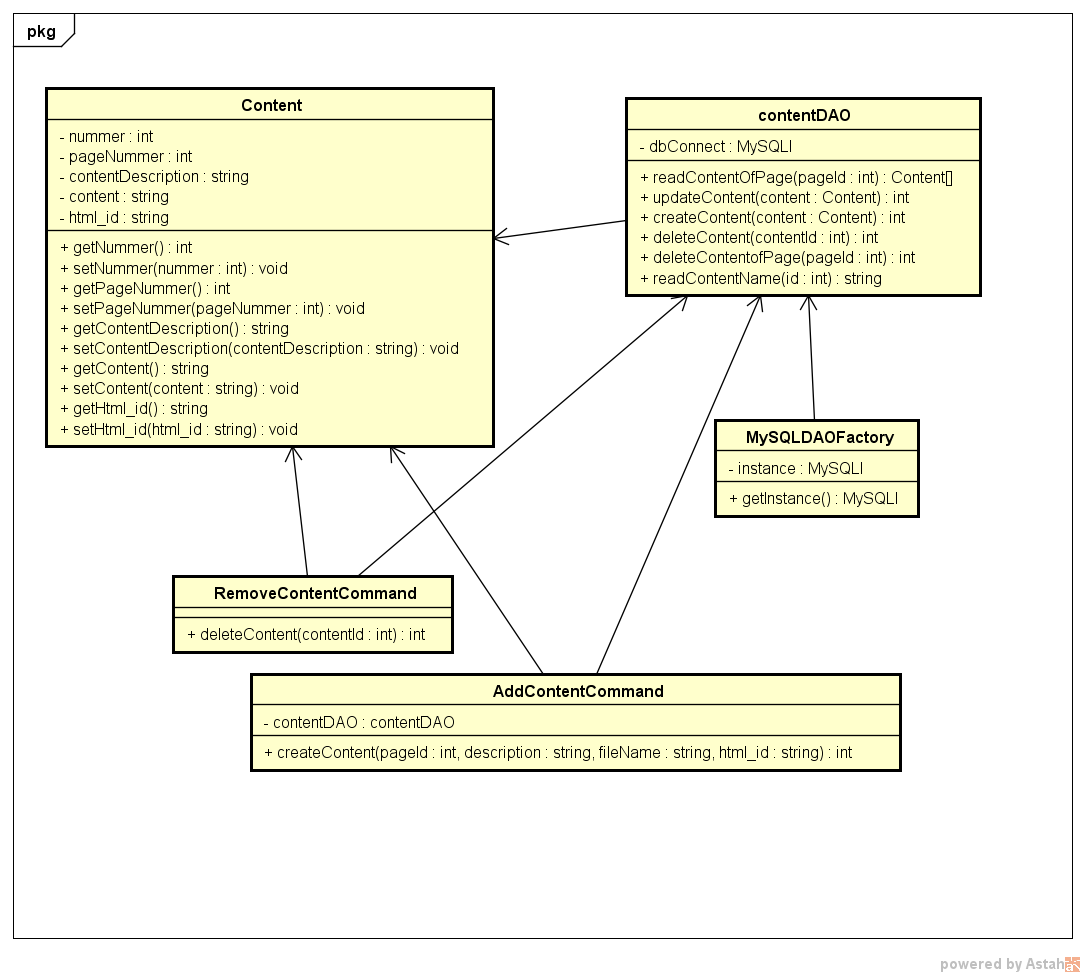
\includegraphics[scale=0.52]{GeschäftsLogik1}
\label{fig:GeschäftsLogik}
\end{figure}

Eine Datenbankverbindung erhalten die Datenmapper UserDAO, PageDAO und ContentDAO über das Singleton MySQLDAOFactory. Ein Singleton ist ein Entwurfsmuster, welches eine statische Eigenschaft enthält,  hier die Verbindung zur Datenbank. Auf diese Eigenschaft kann über eine statische Methode zugegriffen werden. Dabei ist wichtig, dass es nur eine Instanz/ ein Objekt dieser Klasse geben darf.

So werden alle Methoden, die etwas mit der Datenbank zu tun haben, über die Eigenschaft dbConnect aufgerufen. Der Austausch zwischen den Datenzugriffsklassen und den übrigen Komponenten wird über die Standardklassen User, Page und Content gemacht. Entweder wird ein Objekt vom Typ Content übergeben, um einen neuen Inhalt (Content) anzulegen (siehe: Schreiben von neuen Datensätzen) oder es wird zum Lesen ein neues Objekt vom Typ Content angelegt und an die aufrufenden Methode zurückgegeben (siehe: Lesen von Datensätzen).

\textbf{Lesen von Datensätzen:}

\lstset{firstnumber=16}
\begin{lstlisting}
public function readContentOfPage($pageNr){
        $contentList = array();
        $pageNummer = "".$pageNr;
        $sql = "SELECT content.*
                FROM content
                WHERE content.page = ?
                ORDER BY content.id";
        $preStmt = $this->dbConnect->prepare($sql);
        $preStmt->bind_param("s", $pageNummer);
        $preStmt->execute();
		$preStmt->store_result();
        $preStmt->bind_result($id, $page, $content, $description, $html_id);
        
        while($preStmt->fetch()){
			$thisContent = new Content($id, $page, $description, $content, $html_id);

			$contentList[] = $thisContent;
        }
        
        $preStmt->free_result();
        $preStmt->close();
        
        return $contentList;
    }
\end{lstlisting}

\textbf{Schreiben von Datensätzen:}

\lstset{firstnumber=103}
\begin{lstlisting}
public function createContentByCopy(Content $content){

        $pageNummer = (int)$content->getPageNummer();
        $contentDescription = "".$content->getContentDescription();
        $thisContent = "".$content->getContent();
        $html_id = "".$content->getHtml_id();

        $ok = -1;
        $sql = "INSERT INTO content (page, content, description, html_id)
                VALUES (?,?,?,?)";
        $preStmt = $this->dbConnect->prepare($sql);
        $preStmt->bind_param("ssss", $pageNummer, $thisContent, $contentDescription, $html_id);
        $preStmt->execute();
        $ok = $preStmt->insert_id;
        $preStmt->close();
        unset($preStmt);

        return $ok;
    }
\end{lstlisting}

\subsubsection{Programmierung der Controllerklassen}

Über das Front-Controller-Pattern (Anhang D) wird eine zentrale Stelle geschaffen, die Anfragen bearbeitet und an die betreffenden Controller-Klassen weiterleitet.  
Die Command-Control-Schicht hat die Aufgabe eine Anforderung (Request) zu analysieren und die Anfrage mit allen Parametern an den Teil der Anwendung weiterzuleiten, der für die Verarbeitung verantwortlich ist. So erfüllt im Command-Control-Pattern jede Command-Instanz eine spezielle Aufgabe. Eine bestimmte Command-Instanz bearbeitet den Fall, dass vorhandener Content auf Seiten entfernt werden soll (RemoveContentCommand), und eine andere, wenn neuer Content erstellt werden soll (CreateContentCommand).  
Innerhalb der Command-Instanz wird die Verarbeitung an die Businesslogik weitergeleitet, die die Daten verarbeitet, speichert und eventuell ein Ergebnis zurückliefert. Diese Ergebnisse werden als Antwort (Response) an den Browser zurückgeschickt.  
Eingaben werden mittels Request an den Server weitergeleitet. Sämtliche Details zu den Anfragen sind in den beiden Super Globals \textit{\$\_REQUEST} und \textit{\$\_SERVER} gespeichert. Unabhängig von der verwendeten Methode werden alle Name-Werte-Paare in \textit{\$\_REQUEST} zur Verfügung gestellt. Dies ist ein assoziatives Array, welches in allen PHP-Scripten sichtbar ist. Das hei{\ss}t, dass eine URL \textit{index.php?cmd=RemoveContent} innerhalb des Array \textit{\$\_REQUEST} mit \textit{\$\_REQUEST['cmd']} den Wert \textit{RemoveContent} liefert. 
Zuerst werden die Klassen zur Speicherung der Request-Parameter geschrieben.  
Das Interface Request definiert die Methoden:
\begin{itemize}
    \item public function getParameterNames();
	\item public function issetParameter(\$name);
	\item public function getParameter(\$name);
	\item public function getHeader(\$name);
\end{itemize}
Wobei in der konkreten Klasse HttpRequest das ganze \textit{\$\_REQUEST}-Array in der Eigenschaft parameters gespeichert wird, so dass über die Methode getParameter der Wert des einzelnen Eintrags zurückgegeben wird.

\lstset{firstnumber=1}
\begin{lstlisting}
public function getParameter($name){
    if (isset($this->parameters[$name])) {
        return $this->parameters[$name];
    }
    return null;
} 
\end{lstlisting}

Mit textit{\$cmdName = \$request->getParameter("cmd");} wird der Name des nächsten Commands ermittelt. 
Und mit \textit{\$command = \$this->loadCommand(\$cmdName);} die entsprechende Command-Klasse geladen.

Für die verschiedenen Command-Klassen wird wieder ein Interface angelegt, um sicherzustellen, dass jede Command-Klasse die gleiche Methode implementiert. Das Interface enthält nur eine Methodendefinition: 

\begin{lstlisting}
interface Command{
    public function execute(Request $request, Response $response);
} 
\end{lstlisting}

In jeder Command-Implementierung steht der Code, der hier ausgeführt werden soll. Der FrontController lädt die entsprechende Command-Instanz auf und führt genau diese Methode auf. 

\begin{lstlisting}
public function handleRequest(Request $request, Response $response){
    $command = $this->resolver->getCommand($request);
    $command->execute($request, $response);   $response->flush();
}
\end{lstlisting}

Das Interface Response dient den Ausgaben, die dem Benutzer nach der Ausführung der entsprechenden Command-Instanz angezeigt werden sollen.  
In der konkreten Implementierung HttpResponse werden alle Daten, die geschrieben werden an die Eigenschaft body gehängt:

\begin{lstlisting}
public function write($data){
    $this->body .= $data;
} 
\end{lstlisting}

So können innerhalb der Command-Instanzen die Ausgaben mit response->write("   ") getätigt werden. 
Für die Antwort an den Client dient die Methode flush, die alle Inhalte überträgt und die Variablen wieder leert:

\begin{lstlisting}
public function flush(){
    header("HTTP/1.0 " . $this->status);
    foreach ($this->headers as $name => $value){
        header($name . ":" . $value);
    }
    print $this->body;
    $this->headers = array();
    $this->data = null;
}
\end{lstlisting}

\subsubsection{Programmierung der Viewklassen}

\paragraph{Darstellung der Dateien}

Die Seiten und Inhalte eines Benutzers bzw. die ein Gast einsehen darf werden als Arrays im jeweiligen Objekt abgelegt. Diese werden mit \textit{foreach} verarbeitet und abhängig von MIME-Type unterschiedlich dargestellt:

\FloatBarrier
\begin{table}[ht!]
\begin{tabular}{ll}
PDF-Dokumente & Link, der einen neuen Tab im Browser öffnet, in welchem die PDF dargestellt wird \\
Audio-Dateien & Direkt auf der Seite abspielbar \\
Video-Dateien & Direkt auf der Seite abspielbar \\
Alle weiteren & Downloadlink

\end{tabular}
\end{table}
\FloatBarrier

Um den unberechtigten Zugriff zu verhindern, werden die Dateien au{\ss}erhalb des Webroots gespeichert. Damit der Pfad über den Browser nicht ersichtlich ist, wird die Datei in einen base64-String umgewandelt und als URI in den HTML-Code eingefügt.

Als Beispiel befindet sich der Code der UserHome View im Anhang (Listing \ref{lst:UserHome}, Seite \pageref{lst:UserHome})

\subsubsection{Dateiverwaltung}

\paragraph{Dateiupload}

Beim Upload von Dateien durch den Benutzer wird zunächst geprüft, ob es sich auch tatsächlich und eine hochgeladene Datei handelt. Aus Sicherheitsgründen werden danach die MIME-Types der Dateien geprüft und mit einem Array zulässiger Typen verglichen. So wird vermieden, dass der Benutzer Shell-Scripts, php-Scripts usw. hochlädt, selbst wenn er die Dateiendung ändert. Sollte die Datei zulässig sein, wird geprüft, ob bereits eine Datei mit gewählten Namen existiert und ggf. eine Meldung ausgegeben und der Upload abgebrochen. Ist diese Prüfung negativ wird geprüft, ob der Dateiname zulässig ist. Nach aktuellem Stand ist nur der Dateiname "defaultContent" unzulässig. Wenn der Name zulässig ist, wird die Datei in den Ordner des Users verschoben und der Dateiname in der Tabelle \textit{content} eingetragen.

\paragraph{Benutzerordner}

Jeder Bentuzer erhält beim Anlegen einen eigenen Ordner, der nach seiner ID benannt wird. In diesem werden seine Uploads gespeichert. Aus Sicherheitsgründen befindet sich der Benutzerordner au{\ss}erhalb des Webroots um einen ungewollten Zugriff von Au{\ss}en zu verhindern.

\begin{infobox}[Alternative:]
Es kann auch in den Tabellen \textit{user}, \textit{content} und \textit{page} jeweils eine weitere Spalte hinzugefügt werden mit einer zufälligen Folge aus Buchstaben und Zahlen, die eine externe ID darstellen sollen. Dies erhöht nochmals die Sicherheit, da manche Daten über GET in der URL übermittelt werden.
\end{infobox}

\paragraph{Löschen von Dateien}
Will der Benutzer seinen Content löschen, so wird nicht nur der Datesatz aus der Datenbank gelöscht, sonder auch die Datei. Der Benutzer kann somit sicher sein, dass seine Dateien nicht auf ungewollt versteckt verbleiben. Hierzu wird zunächst ermittelt welches Betriebssystem auf dem Server läuft um mit dem korrekten Befehl die Datei zu entfernen:

\lstset{firstnumber=53}
\begin{lstlisting}
if(strtoupper(substr(PHP_OS, 0, 3)) === 'WIN') {
    unlink(USERS_DIR . $currentUser->getId() . '/' . $file);
} else {
    shell_exec('rm ' . USERS_DIR . $currentUser->getId() . '/' . $file);
}
\end{lstlisting}

\paragraph{Verhalten bei Accountlöschung}
Möchte der Benutzer seinen Account vollständig löschen, so werden alle seine Dateien sowie sein Benutzerordner vom System gelöscht. Um dies sicherzustellen wird auch hier zuerst das Betriebssystem ermittelt. Bei Windows wird zunächst jede Datei einzeln gelöscht um anschlie{\ss}end den Ordner zu entfernen. Bei Linux Systemen sowie BSD und anderen unixoiden System kann der Ordner samt Inhalt mit einem an die Shell übergebenem Befehl gelöscht werden:

\lstset{firstnumber=31}
\begin{lstlisting}
if(strtoupper(substr(PHP_OS, 0, 3)) === 'WIN') {
    foreach (glob(USERS_DIR . $userId . "/*.*") as $filename) {
        unlink($filename);
    }
    rmdir(USERS_DIR . $userId);
} else {
    shell_exec('rm -rf ' . USERS_DIR . $userId);
}
\end{lstlisting}
Als Beispiel befindet sich der vollständige Code zur Accountlöschung durch den Admin im Anhang (Listing \ref{lst:RemoveUserCommand}, Seite \pageref{lst:RemoveUserCommand}).

\subsection{Tests}

\begin{table}[ht!]
\begin{tabularx}{\textwidth}{l | l}

\textbf{Test}  & \textbf{Ergebnis}\\
\hline
Selber Gast von zwei Benutzern  & Der Gast kann sich mit zwei verschiedenen Passwörtern anmelden\\
s. o. mit gleichem Passwort & Gast kann sich die Portfolios aussuchen, die er sehen will\\
Anmeldung ohne Validierung & nicht möglich, Gast muss seine Adresse erst validieren\\

\end{tabularx}
\end{table}

\section{Soll-/Ist-Vergleich}

Folgende Musskriterien wurden implementiert:

\begin{itemize}
	\item Neuanlegen, bearbeiten und löschen von Benutzern durch den Admin
	\item Jeder Benutzer hat eine Seite, die nur er bearbeiten kann
	\item Anlegen, bearbeiten und löschen von Texten und Links
	\item Upload von Dateien (Bilder, Dokumente)
	\item nur registrierte Gäste mit validierter Adresse können die Portfolios einsehen.
\end{itemize}

Folgende Wunschkriterien wurden implementiert:

\begin{itemize}
	\item Gäste können nur für sie freigegebene Portfolios einsehen
\end{itemize}

Es konnten alle Kriterien implementiert werden. Der Code ist erweiterbar und lässt weitere Implementierungen zu, wenn der Kunde dies wünscht.

\section{Fazit}

Die Entwicklung des ePortfolios ermöglicht einen ersten Einblick in den Aufbau und Struktur von Social Media Seiten. Einer der wichtigsten Aspekte bei der Entwicklung stellt die Sicherheit dar und die jeweiligen Tests um diese zu erhöhen. Bei der Entwicklung ist uns aufgefallen, dass man sehr viele Optionen implementieren kann um den User grö{\ss}tmögliche Individualität zu ermöglichen. Auch beim Design gibt es sehr viel Spielraum, der ein erfahrener Webdesign nutzen kann um den Benutzer ein optisch ansprechendes Portfolio zu bieten, mit welchem er sich bei Kunden und potenziellen Arbeitgeber präsentieren kann.

\newpage
\section{Anhang}
\subsection{Code Listings}

\lstset{firstnumber=1, basicstyle=\footnotesize}

\begin{lstlisting}[caption={UserHome.php}, label={lst:UserHome}]
<!DOCTYPE html>
<html lang="en">
    <head>
        <meta charset="UTF-8">
        <meta name="viewport" content="width=device-width, initial-scale=1.0">
        <title>Document</title>
        <link href="./css/<?= $this->style ?>.css" rel="stylesheet" type="text/css">
        <link rel="shortcut icon" type="image/x-icon" href="./favicon_96x96.png" size="48x48">
    </head>
    <body>
        <div id="header">
            Das ePortfolio von <?= $this->displayname ?>!
        </div>
        <ul>
            <?php 
                $indexOfPageList = 0;
                foreach($this->pageList as $page) {
                     echo '<li><a href="./index.php?cmd=UserHome&page='.$indexOfPageList.'">'. $page->getTitle() ."</a></li>"; 
                     $indexOfPageList++;
                }
            ?>
            <li><a href="./index.php?cmd=AddPage">±</a></li>
            <li style="float: right"><a href="index.php?cmd=Logout">Logout</a></li>
            <li style="float: right"><a href="./index.php?cmd=UserSettings">Einstellungen</a></li>
        </ul>
        <div id="main">

            <h2><?= $this->requestedTitle ?></h2>
            <?= $this->alert ?>
            <?= $this->editLink ?><br>
            <?= $this->addContentLink ?>

            <?php

                $output = "";
                foreach($this->requestedContent as $content) {

                    if(!$content->getContent() == null) {
                        $file = $this->filepath . $content->getContent();

                        if(file_exists($file)) {

                            $mimeType = mime_content_type($file);

                            $tmp = base64_encode(file_get_contents($file));

                            if(!strstr($mimeType, "image") == false) {
                                $output = '<a href="data:'.$mimeType.';base64,'.$tmp.'" target="_blank"><img src="data:'.$mimeType.';base64,'.$tmp.'"></a><br><br>';
                            } else if(!strstr($mimeType, "audio") == false) {
                                $output = '<audio controls><source src="data:'.$mimeType.';base64,'.$tmp.'" type="'.$mimeType.'">Der Browser unterstütz das Format '.$mimeType.' nicht!</audio><br><br>';
                            } else if(!strstr($mimeType, "video") == false) {
                                $output = '<video controls><source src="data:'.$mimeType.';base64,'.$tmp.'" type="'.$mimeType.'">Der Browser unterstütz das Format '.$mimeType.' nicht!</video><br><br>';
                            } else {
                                $output = '<a href="data:'.$mimeType.';base64,'.$tmp.'" target="_blank">'. $content->getContent() .'</a><br><br>';
                            }
                        }
                    } else {
                        $output = "";
                    }
                    echo "<div id='content'>" . $output . $content->getContentDescription() . "<br></div>";
                }
            ?>
        </div>
        <footer>&copy; 2020 M. Mandler & D. Zielke</footer>
    </body>
</html>
\end{lstlisting}


\begin{lstlisting}[caption={RemoveUserCommand.php}, label={lst:RemoveUserCommand}]
<?php
    namespace classes\commands;

    use classes\request\Request;
    use classes\response\Response;
    use classes\template\HtmlTemplateView;
    use classes\mapper\UserDAO;
    use classes\model\User;

    class RemoveUserCommand implements Command{
        public function execute(Request $request, Response $response) {

            if (isset($_SESSION['admin'])){
                $currentUser = unserialize($_SESSION['admin']);
            } else {
                header('location: index.php');
            }             
            if (!($currentUser instanceof User)){
                header('location: index.php');
            }            
            if ($currentUser->getStatus() != "admin"){
                header('location: index.php');
            }
            
            $userDAO = new UserDAO;

            if($request->issetParameter('deleteUser')) {
                $userId = $request->getParameter('deleteUser');
                $userDAO->deleteUser($userId);

                if(strtoupper(substr(PHP_OS, 0, 3)) === 'WIN') {
                    foreach (glob(USERS_DIR . $userId . "/*.*") as $filename) {
                        unlink($filename);
                    }
                    rmdir(USERS_DIR . $userId);
                } else {
                    shell_exec('rm -rf ' . USERS_DIR . $userId);
                }
            }

            $listOfAllUsers = $userDAO->readAllUsersWithPages("user");
            $multiListArray = array();
            for($i = 0; $i < count($listOfAllUsers); $i++){
                $multiListArray[$i][] = $listOfAllUsers[$i];
                $multiListArray[$i][] = $userDAO->readGuestListOfUser($listOfAllUsers[$i]->getId());
            }

            $view = 'RemoveUser';
            $template = new HtmlTemplateView($view);
            $style = "default"; // provisorisch
            $template->assign('style', $style);
            $template->assign('userList', $multiListArray);
            $template->render( $request, $response);
        }
    }
?>
\end{lstlisting}

\newpage
\subsection{Abbildungen}

\begin{figure}[h!]
\caption{Datenmodell}
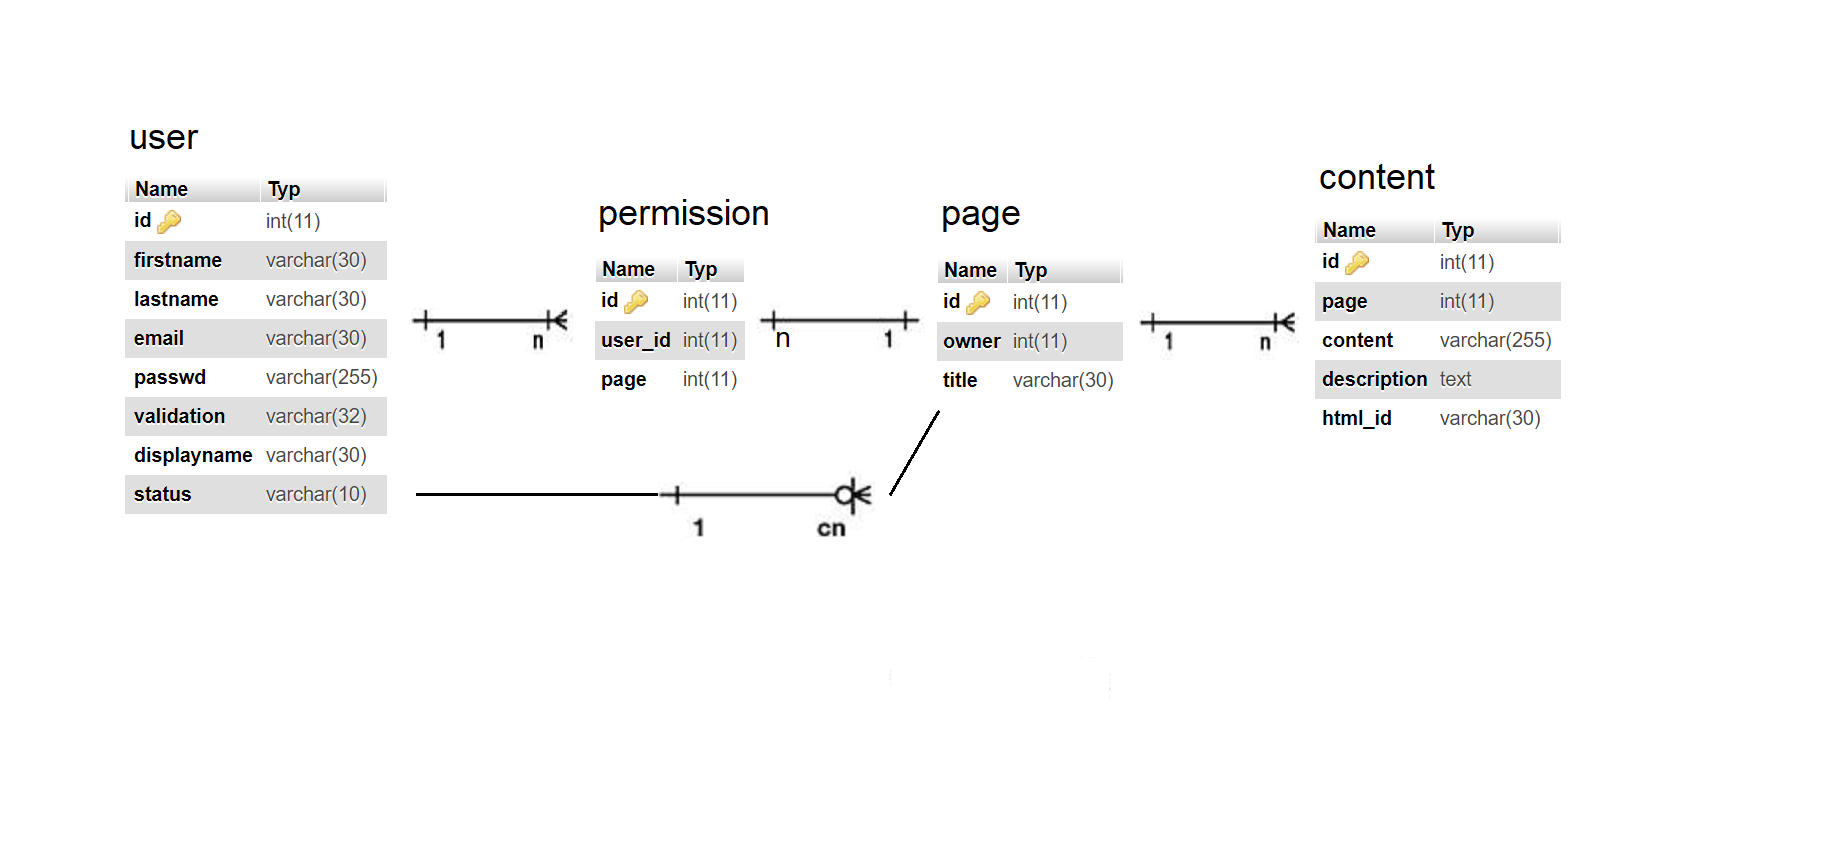
\includegraphics[width=\textwidth]{DatenmodellEPortfolio}
\label{fig:datenmodell}
\end{figure}

\begin{figure}[h!]
\caption{Klassendiagramm}
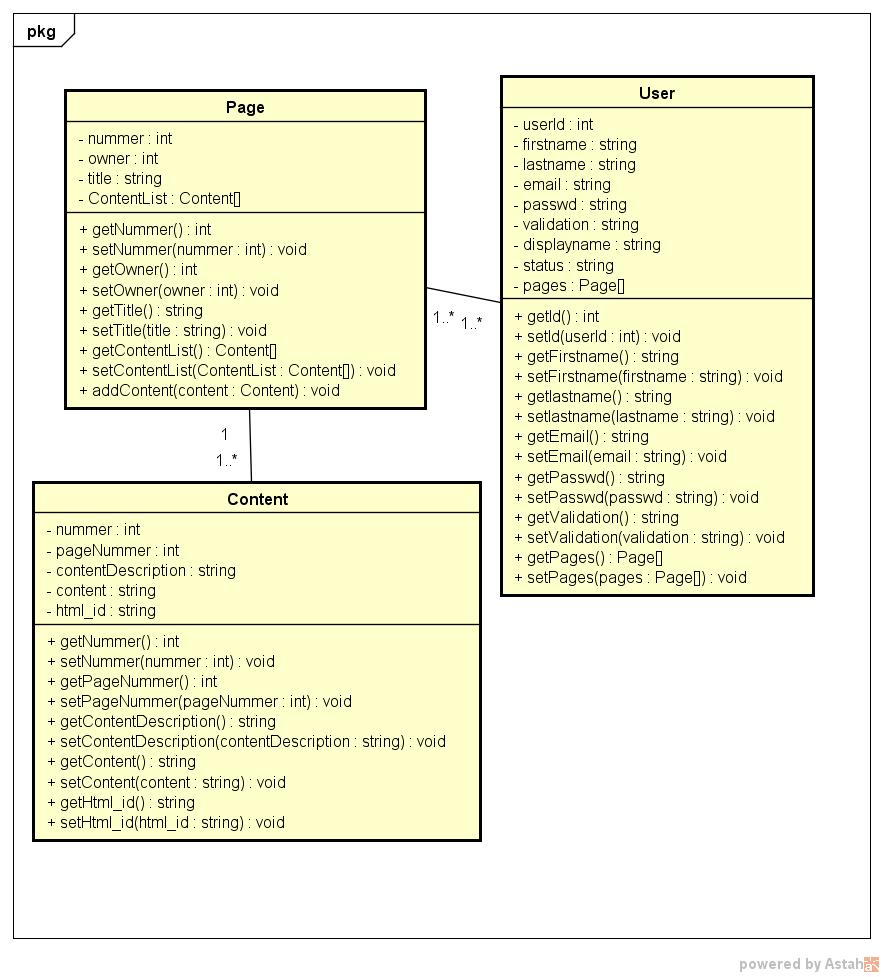
\includegraphics[scale=0.35]{ClassDiagram}
\label{fig:classdiagram}
\end{figure}

\begin{figure}[h!]
\caption{Use Case Diagram}
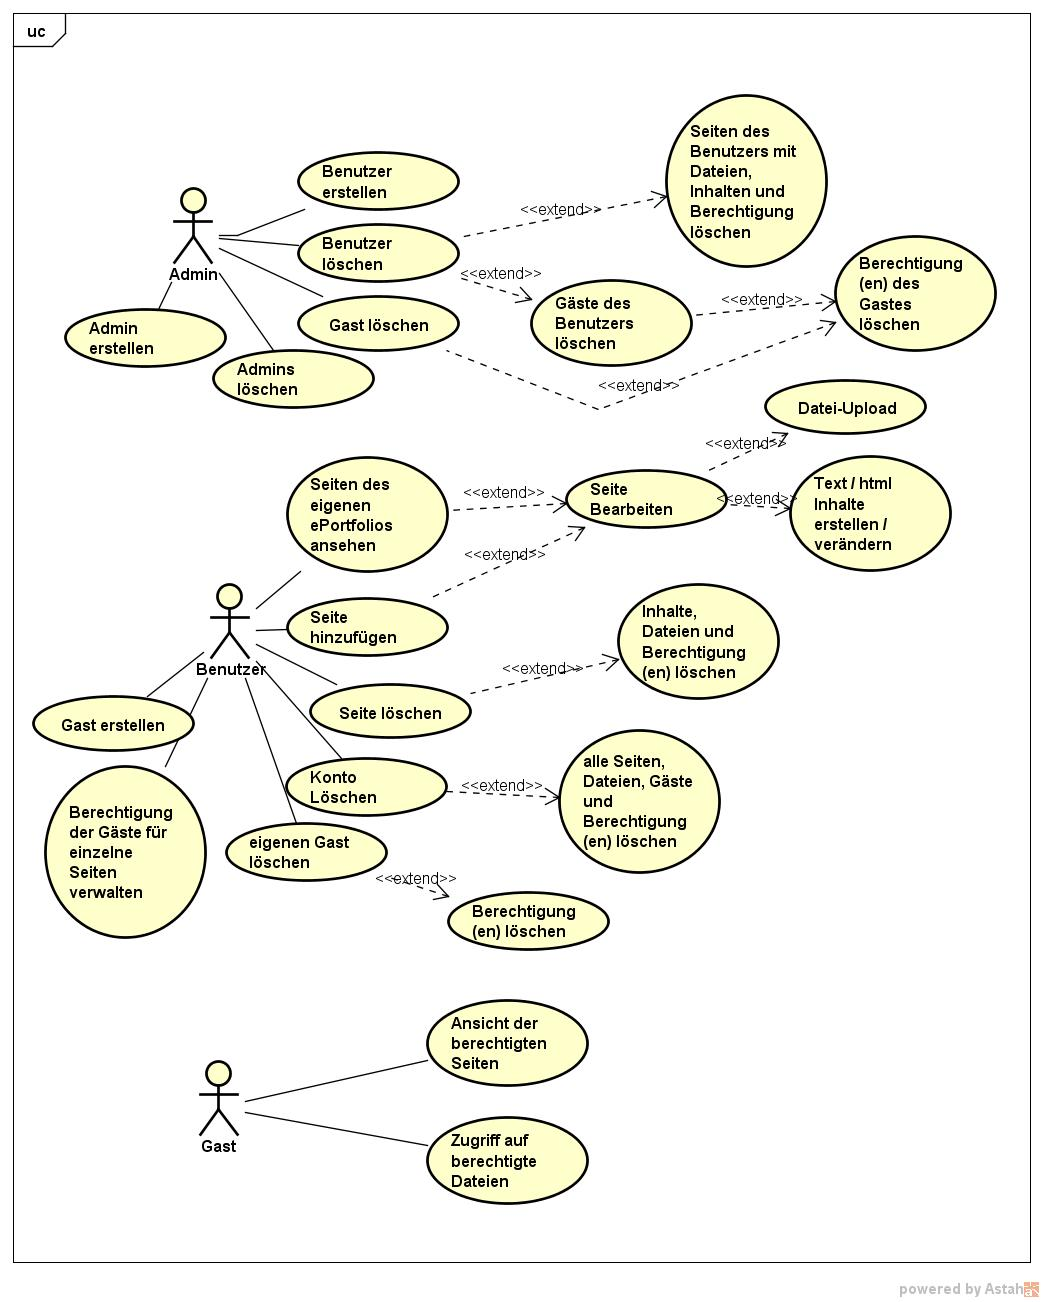
\includegraphics[width=\textwidth]{UseCaseDiagram}
\label{fig:usecasediagram}
\end{figure}

\end{document}